\documentclass[a4paper]{article}
\usepackage[14pt]{extsizes} % для того чтобы задать нестандартный 14-ый размер шрифта
\usepackage[margin=0.7in]{geometry}
\usepackage{multirow}
\usepackage {graphicx}
\usepackage[utf8x]{inputenc} % указать кодировку русского текста
\usepackage[russian]{babel} % указать, что язык текста - русский
\usepackage{fancyhdr}
\pagestyle{fancy}
\usepackage{graphicx}
\graphicspath{{pictures/}}
\DeclareGraphicsExtensions{.pdf,.png,.jpg}
\usepackage{tocloft}
\renewcommand{\cftsecleader}{\cftdotfill{\cftdotsep}}
\begin{document} 
 \begin{titlepage}
\begin{center}
\hfill \break
Министерство науки и высшего образования Российской Федерации\\
ФЕДЕРАЛЬНОЕ ГОСУДАРСТВЕННОЕ АВТОНОМНОЕ ОБРАЗОВАТЕЛЬНОЕ\\ 
УЧРЕЖДЕНИЕ ВЫСШЕГО ОБРАЗОВАНИЯ\\ 
«МОСКОВСКИЙ ФИЗИКО-ТЕХНИЧЕСКИЙ ИНСТИТУТ\\ 
(НАЦИОНАЛЬНЫЙ ИССЛЕДОВАТЕЛЬСКИЙ УНИВЕРСИТЕТ)»\\
(МФТИ)\\
\hfill \break
\hfill \break
\hfill \break
\hfill \break
\hfill \break
\hfill \break
\hfill \break
\hfill \break
\hfill \break
\hfill \break
\hfill \break
КАФЕДРА ВАКУУМНОЙ ЭЛЕКТРОНИКИ\\
\hfill \break
ОТЧЕТ\\
ПО ЛАБОРАТОРНОЙ РАБОТЕ\\
\hfill \break
МЕТОДЫ ПОЛУЧЕНИЯ ВЫСОКОГО ВАКУУМА\\
\end{center}
\hfill \break
\hfill \break
\hfill \break
\hfill \break
\hfill \break
\hfill \break
\hfill \break
\hfill \break
\begin{tabular}{ccc}
Работу выполнили студенты  & \underline{\hspace{3cm}}& П.Ю. Шлыков \\\\
группы Б04-004& \underline{\hspace{3cm}}& М.В. Шлапак  \\\\
 & \underline{\hspace{3cm}}& Н.А. Плюскова  \\\\
Работу принял, оценка & \underline{\hspace{3cm}} &  \\\\
\end{tabular}
\hfill \break
\hfill \break
\begin{center} Долгопрудный 2021 \end{center}
\end{titlepage}
\fancyhead[L] {Методы получения высокого вакуума}
\tableofcontents    
\newpage
\normalsize
\section{Цель работы}
\begin{enumerate}
    \item Ознакомиться с принципом работы форвакуумного насоса.
    \item Ознакомиться с методами вакуумных расчётов, найти зависимость величины газового потока в системе от давления.
    \item Определить производительность турбомолекулярного насоса.
    \item Рассчитать объем рабочей камеры.
\end{enumerate}

\section{Лабораторная установка}

Лабораторная установка предназначена для ознакомления с основными приборами вакуумной техники: насосами, манометрами, измерителями расхода газа. Схема установки представлена на рисунке 1.
\begin{figure}[h]
    \centering
    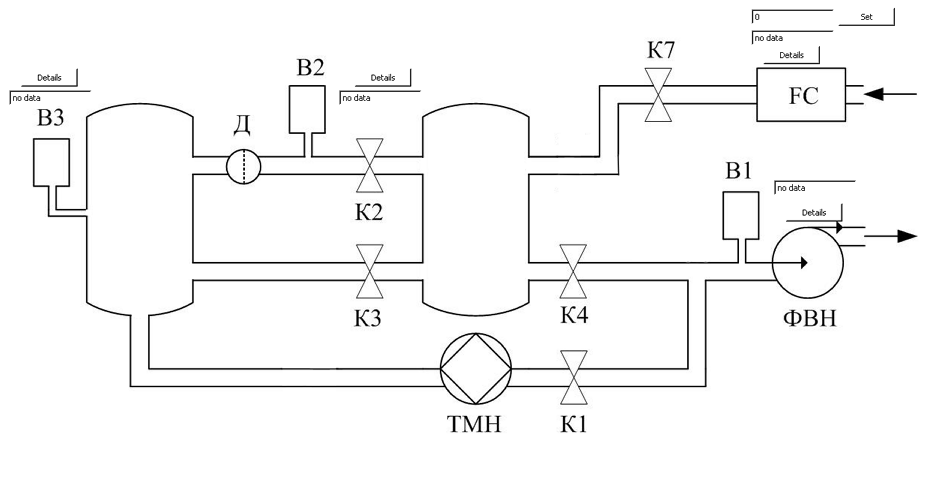
\includegraphics[width=\textwidth]{facility.PNG}
    \caption{Схема лабораторной установки}
    \label{fig:vac}
\end{figure}

На схеме обозначены: \\
$B_1$ - вакуумметр ёмкостной\\
$B_2$ - вакуумметр терморезисторный\\
$B_3$ - вакуумметр ионизационный\\
$K_1$ - кран турбомолекулярного насоса\\
$K_3$ - высоковакуумная заслонка\\
$K_4$ - форвакуумная заслонка\\
$K_2, K_7$ - коммутационные краны\\
Д - диафрагма\\
FC - регулятор газового потока (flow controller)\\
ТМН - турбомолекулярный насос\\
ФВН - форвакуумный насос\\

\section{Выполнение работы}
\subsection{Подготовка к экспериментам}
\begin{enumerate}
    \item Включаем компьютер, монитор, контроллер, загружаем операционную систему.
    \item Открываем все клапаны в вакуумной системе - К2, К3, К4, К7.
    \item Полностью откручиваем, снимаем и затем закручиваем на место до полного уплотнения клапан напуска атмосферы и убеждаемся, что в систему напущен воздух.
    \item Создаем все необходимые для сохранения графиков папки на компьютере.
    \item Запускаем C:|vacuum|SCADA$\_$client.exe.
    \item Включаем в программе вакууметры В1 и В2, регулятор расхода газа FC.
    \item делаем запись в лабораторном журнале, чтобы впоследствии синхронизировать начало отсчёта для всех графиков.
\end{enumerate}
\textbf{ Начальное состояние системы: все клапаны открыты, давление внутри системы - атмосферное. 16:23 - включены вакууметры В1, В2 и регулятор расхода газа FC.}\\
\subsection{Эксперимент 1. Откачка вакуумной системы с помощью форвакуумного насоса.}
\textbf{16:23 - время включения форвакуумного насоса}\\
В течение 10 минут давление в $10^{-2}$ Торр достигнуто не было, из чего можно сделать вывод, что установка чисто физически не может откачать до такого давления.\\
\textbf{16:34 - прекращение эксперимента}\\

\subsection{Эксперимент 2. Откачка вакуумной системы с газовой нагрузкой.}
При давлении примерно 0.02 Торр получили $\triangle Q \approx 2.2 sccm $, что по нашей оценке равно натеканию газа на нашей установке. Можно предположить, что датчик на регуляторе потока показывает значение потока сразу с учётом натекания. $Q_{leak} + Q_{FC} = Q$

Поток воздуха 
\begin{center}
$Q-P*S(P)=\frac{d(PV)}{dt}$
\end{center}
При $P = const$
\begin{center}
$\frac{d(PV)}{dt}=0$
\end{center}
Тогда
\begin{center}
$S(P)=\frac{Q}{P}$
\end{center}

По этой формуле рассчитаем значения S(P) и занесём результаты в таблицу 1. Построим график зависимости Q от P (рисунок 5), тогда по формуле среднее значение S будет равно угловому коэффициенту получившейся прямой, переведённой в $m^3/h$. 
\begin{center}
$S = 95.242 sccm = 4.33 m^3/h$
\end{center}

Но рассчитанные значения не совпадают с этой аппроксимацией. Значит, имеется другой характер зависимости.
Быстродействие насоса также зависит от давления в установке.

\begin{center}
$Q = \frac{d(PV)}{dt}$\\
$S(P) = \frac{Q}{P}=-V\frac{d(lnP)}{dt}$\\
$P(t) = P_0+P(0)*exp(\frac{S_0}{V}*t)$\\
$S(P) = S_0(1-\frac{P_0}{P})$
\end{center}

По значениям из таблицы 1 построим график зависимости быстродействия от давления в установке (рисунок 6). Экстраполируем его под полученную зависимость: $S_0 = 3.65 m^3/h, P_0 = 0.02 torr$. Полученное значение на 16\% отличается от экстраполированного по прямой.

\subsection{Эксперимент 3. Высоковакуумная откачка.}

\begin{enumerate}
\item Закроем К3, включаем турбомолекулярный насос.\\
\textbf{16:51 - время включения турбомолекулярного насоса}
\item Убеждаемся, что турбомолекулярный насос вышел на рабочий режим  42000 об/мин. (зелёный диод горит непрерывно).
\item Включаем вакууметр В3.\\
\textbf{ 16:53 - время включения вакууметра В3}
\item Дожидаемся резкого излома на графике показаний вакууметра В3.\\
\textbf{17:01 - появление резкого излома на графике показаний вакууметра В3}
\item Поднимаем давление в форвакуумной части системы до давления примерно 1 Торр по схеме:
\begin{enumerate}
\item устанавливаем поток 5 sccm
\item ждем 10 секунд
\item устанавливаем поток 10 sccm
\item ждем 10 секунд
\item устанавливаем поток 15 sccm
\item ждем 10 секунд
\item устанавливаем поток 20 sccm
\item ждем 10 секунд
\item устанавливаем поток 25 sccm
\item ждем 10 секунд
\item устанавливаем поток 30 sccm
\item ждем 10 секунд
\item устанавливаем поток 35 sccm
\item ждем 10 секунд
\item устанавливаем поток 40 sccm
\item ждем 10 секунд
\end{enumerate}
\item Закрываем клапан К2.
\item Отключаем подачу газа в систему.\\
\textbf{17:03 - время закрытия К2. Установлен поток газа, равный нулю.}
\item Определим, можно ли считать течение газа через диафрагму молекулярным. Для этого оценим длину свободного пробега молекул:
\begin{center}
$\lambda = \frac{kT}{\sigma P} \approx 1.22m$
\end{center}
где $k = 1,38 \cdot 10^{-23}$ Дж/К – постоянная Больцмана\\
      $T \approx 293$ К – комнатная температура\\
       $\sigma = 62,5 \cdot 10^{-20} m^2$ – среднее эффективное сечение рассеяния для воздуха\\
       $P \approx 4 \cdot 10^{-5}$ Торр = $4 \cdot 133 \cdot 10^{-5}$ Па – порядок давления в высоковакуумной части системы\\

Диаметр отверстия диафрагмы равен d = 100 мкм. Видно, что $d \ll \lambda$, поэтому течение газа через диафрагрму можно считать молекулярным. Следовательно, справедлива формула нахождения молекулярного потока через диафргаму (отверстие):
\begin{center}
$Q = S\sqrt{\frac{RT}{2\pi\mu}}(P_2-P_3)$
\end{center}
где $P_2, P_3$ - давления на В2 и В3 соответственно\\
$S = \frac{\pi d^2}{4}$ - площадь отверстия в диафрагме\\
$\mu$ - молярная масса воздуха

Так как $P_3 \\ll P_2$, формула примет вид
\begin{center}
$Q = \frac{\pi d^2}{4}\sqrt{\frac{RT}{2\pi\mu}}P_2$
\end{center}
\item Рассмортим модель потока через турбомолекулярный насос
\begin{center}
$P_3S(P_3) = Q - \frac{d(P_2V)}{dt}$\\
$Q \gg \frac{d(P_2V)}{dt}$
\end{center}
Получим:
\begin{center}
$P_3S(P_3) = Q = \frac{\pi d^2}{4}\sqrt{\frac{RT}{2\pi\mu}}P_2$
\end{center}

\item Построим по полученным данным график зависимости давления от времени в высоковакуумной части при включенном турбомолекулярном насосе, а также график зависимости производительности турбомолекулярного насоса от впускного давления. Расчитаем поток через диафрагму (график зависимости потока от времени).

\item Сравним это значение с данными производителя: график зависимости производительности от давления при разных газах представлен на рисунке 10
  \begin{figure}[h]
    \centering
    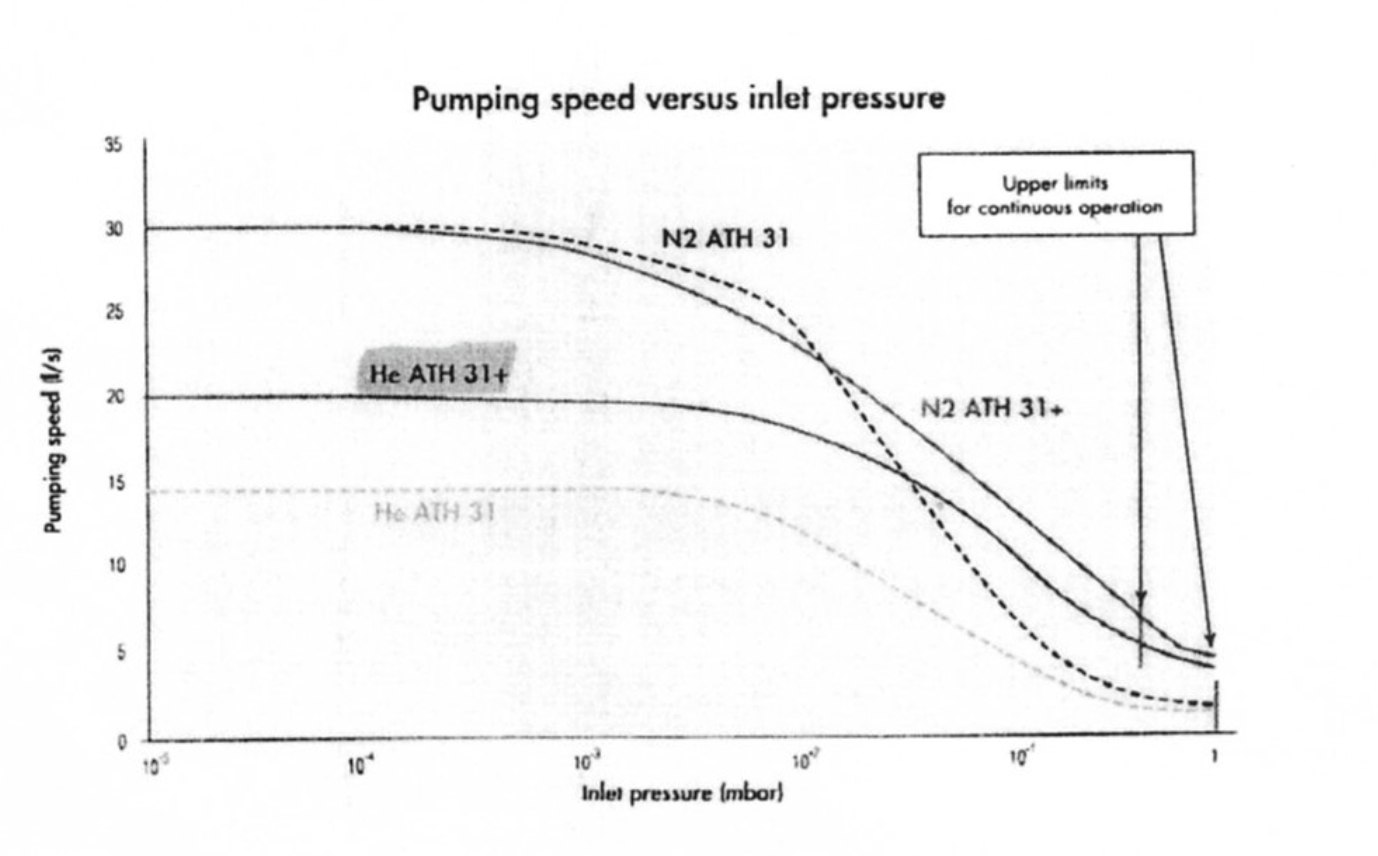
\includegraphics[width=13cm]{man_data.jpg}
    \caption{Данные производителя о зависимости производительности тМН от давления}
    \label{fig:vac}
\end{figure}

По документации производительность ТМН, перекачивающего азот (основная часть атмосферы), равна 30 л/с при давлениях порядка $10^{-5}$ Торр и практически постоянна. Турбомолекулярный насос в нашем эксперименте быстро вышел на свои предельные значения при $10^{-5}$ Торр и рассчитанная производительность практически совпадает с данными производителя.

\item Для определения объёма рабочей камеры необходимо создать условия отсутствия натекания газа через диафрагму. В нашем эксперименте таких условия предоставлено не было, следовательно, нельзя с большой точность определить объём рабочей камеры
\end{enumerate}

\section {Вывод}
В ходе работы мы ознакомились с принципами работы вакуумной техники, определили характеристики насосов и вакуумметров, изучили методы получения и измерения вакуума. 
\begin{enumerate}
\item Определены рабочие диапазоны вакуумметров:
\begin{itemize}
  \item ёмкостной:$760 - 1$ Торр
  \item терморезисторный: $10 - 10^{-3} $ Торр
  \item ионизационный: $10^{-3} - 10^{-5}$ Торр
\end{itemize}
\item На установке получен высокий вакуум порядка $10^{-5}$ Торр
\item Определены быстродействия вакуумных насосов:
\begin{itemize}
  \item форвакуумный: $3.65 m^3/h$
  \item турбомолекулярный $26.1 m^3/h$: 
\end{itemize}
\end{enumerate}

\section{Список использованной литературы}
\begin{enumerate}
\item Методы получения высокого вакуума: лабораторная работа по курсу Вакуумная электроника / сост.: А.С. Батурин, И.Н. Ескин, Д.А. Свинцов, П.А. Стариков, Е.П. Шешин – М.: МФТИ, 2010. – 36 с.
\item Шешин Е.П. — Основы вакуумной электроники: учеб. пособие. – 2-е издание, испр. И доп. - М.: МФТИ, 2009.  - 149 с.
\item Шешин Е.П. — Вакуумные технологии: учеб. пособие. / 
Долгопрудный: издательский Дом «Интеллект», 2009.  - 504 с.
\end{enumerate}
\end{document}  